\documentclass[11pt,a4paper]{article}
\usepackage[utf8]{inputenc}
\usepackage[T1]{fontenc}
\usepackage{amsmath,amsfonts,amssymb}
\usepackage{graphicx}
\usepackage{tikz}
\usetikzlibrary{shapes,arrows,positioning,calc,decorations.pathreplacing}
\usepackage{hyperref}
\usepackage{geometry}
\geometry{margin=1in}
\usepackage{listings}
\usepackage{xcolor}
\usepackage{float}

\title{OpenCV Similarity Matching for Doodle Recognition: A Feature-Based Approach}
\author{Doodle Recognition Project}
\date{\today}

\begin{document}

\maketitle

\tableofcontents
\newpage

\section{Introduction}

This document explains how OpenCV-based similarity matching works for recognizing doodles from the QuickDraw dataset. Unlike deep learning approaches (ResNet, CNNs), this method uses traditional computer vision techniques built into OpenCV's cv2 library, achieving recognition through direct image-to-image comparison without neural networks.

The implementation combines three complementary methods:
\begin{itemize}
    \item \textbf{Template Matching}: Normalized correlation-based comparison
    \item \textbf{Feature Matching}: Keypoint detection and descriptor matching (SIFT/ORB)
    \item \textbf{Histogram Comparison}: Statistical distribution matching
\end{itemize}

\section{Fundamentals of Similarity-Based Recognition}

\subsection{The Core Concept}

Unlike neural networks that learn abstract features, similarity matching works on a simple principle:
\begin{quote}
\textit{``Compare the test image directly with reference images from each category, and choose the category with the highest similarity score.''}
\end{quote}

This is analogous to how a human might recognize a doodle by comparing it to mental templates of different objects.

\subsection{Image Representation}

Just like with ResNet, a doodle is represented as a matrix of pixel values:
\begin{itemize}
    \item \textbf{Input}: $64 \times 64$ grayscale matrix (values 0-255)
    \item \textbf{Preprocessing}: Invert if needed (ensure dark strokes on light background)
    \item \textbf{Normalization}: Scale to range [0, 1] for comparison
\end{itemize}

\subsection{The Similarity Matching Pipeline}

\begin{figure}[H]
\centering
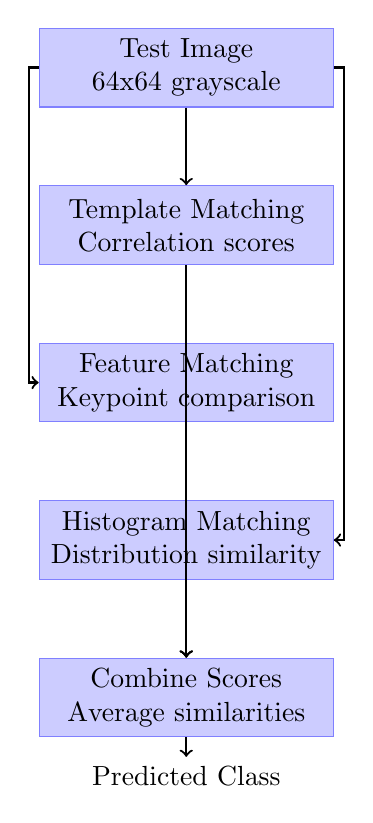
\begin{tikzpicture}[
    node distance=2.0cm,
    box/.style={rectangle, draw=blue!50, fill=blue!20, minimum width=3.5cm, minimum height=1cm, text centered},
    arrow/.style={->, thick}
]

% Pipeline steps
\node[box, text width=3.5cm, align=center] (input) {Test Image\\64x64 grayscale};

\node[box, text width=3.5cm, align=center, below of=input] (template) {Template Matching\\Correlation scores};

\node[box, text width=3.5cm, align=center, below of=template] (features) {Feature Matching\\Keypoint comparison};

\node[box, text width=3.5cm, align=center, below of=features] (histogram) {Histogram Matching\\Distribution similarity};

\node[box, text width=3.5cm, align=center, below of=histogram] (combine) {Combine Scores\\Average similarities};

\node[below of=combine, node distance=1cm] (output) {Predicted Class};

% Arrows
\draw[arrow] (input) -- (template);
\draw[arrow] (input) -| +(-2,0) |- (features);
\draw[arrow] (input) -| +(2,0) |- (histogram);
\draw[arrow] (template) -- (combine);
\draw[arrow] (features) -- (combine);
\draw[arrow] (histogram) -- (combine);
\draw[arrow] (combine) -- (output);

\end{tikzpicture}
\caption{Multi-Method Similarity Matching Pipeline}
\label{fig:pipeline}
\end{figure}

\section{Method 1: Template Matching}

\subsection{What is Template Matching?}

Template matching slides a reference image (template) over the test image and computes similarity at each position. OpenCV provides \texttt{cv2.matchTemplate()} with multiple correlation methods.

\subsection{Normalized Cross-Correlation}

The primary method used is \textbf{TM\_CCOEFF\_NORMED} (normalized correlation coefficient):

\begin{equation}
R(x,y) = \frac{\sum_{x',y'} (T(x',y') \cdot I(x+x', y+y'))}{\sqrt{\sum_{x',y'} T(x',y')^2 \cdot \sum_{x',y'} I(x+x',y+y')^2}}
\end{equation}

Where:
\begin{itemize}
    \item $T$ = Template image
    \item $I$ = Test image
    \item $R(x,y)$ = Correlation score at position $(x,y)$
    \item Range: $[-1, 1]$, where 1 = perfect match
\end{itemize}

\subsection{Template Matching Visualization}

\begin{figure}[H]
\centering
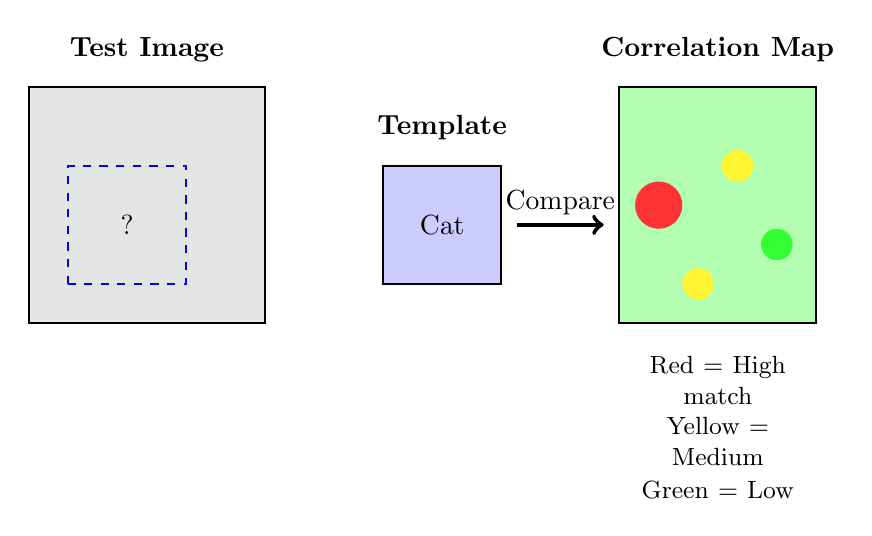
\begin{tikzpicture}[scale=1.0]

% Test image
\draw[thick, fill=gray!20] (0,0) rectangle (3,3);
\node[above] at (1.5, 3.2) {\textbf{Test Image}};
\draw[blue, thick, dashed] (0.5, 0.5) rectangle (2, 2);
\node at (1.25, 1.25) {?};

% Template
\draw[thick, fill=blue!20] (4.5,0.5) rectangle (6,2);
\node[above] at (5.25, 2.2) {\textbf{Template}};
\node at (5.25, 1.25) {Cat};

% Arrow
\draw[->, ultra thick] (6.2, 1.25) -- (7.3, 1.25);
\node[above] at (6.75, 1.25) {Compare};

% Result
\draw[thick, fill=green!30] (7.5, 0) rectangle (10, 3);
\node[above] at (8.75, 3.2) {\textbf{Correlation Map}};

% Heat map representation
\fill[red!80] (8, 1.5) circle (0.3);
\fill[yellow!80] (8.5, 0.5) circle (0.2);
\fill[yellow!80] (9, 2) circle (0.2);
\fill[green!80] (9.5, 1) circle (0.2);

\node[below, text width=2.5cm, align=center] at (8.75, -0.3) {\small Red = High match\\Yellow = Medium\\Green = Low};

\end{tikzpicture}
\caption{Template matching produces a correlation map showing similarity at each position}
\label{fig:template_match}
\end{figure}

\subsection{How It Works for Doodles}

For each category:
\begin{enumerate}
    \item Create a \textbf{mean template} from training samples
    \item Normalize both test image and template to [0, 1]
    \item Apply \texttt{cv2.matchTemplate()} with TM\_CCOEFF\_NORMED
    \item Take maximum correlation score
    \item Also test with TM\_CCORR\_NORMED and average results
\end{enumerate}

\section{Method 2: Feature Matching}

\subsection{Keypoint Detection}

Feature matching detects distinctive points (keypoints) in the image and compares their descriptors.

\subsubsection{SIFT (Scale-Invariant Feature Transform)}

SIFT detects keypoints that are invariant to:
\begin{itemize}
    \item Scale changes (zooming)
    \item Rotation
    \item Illumination changes
    \item Minor viewpoint changes
\end{itemize}

Each keypoint is described by a 128-dimensional vector capturing local gradient information.

\subsubsection{ORB (Oriented FAST and Rotated BRIEF)}

If SIFT is unavailable (requires opencv-contrib-python), ORB is used:
\begin{itemize}
    \item Faster than SIFT
    \item Binary descriptors (256 bits)
    \item Rotation invariant
    \item Free and open-source
\end{itemize}

\subsection{Feature Matching Process}

\begin{figure}[H]
\centering
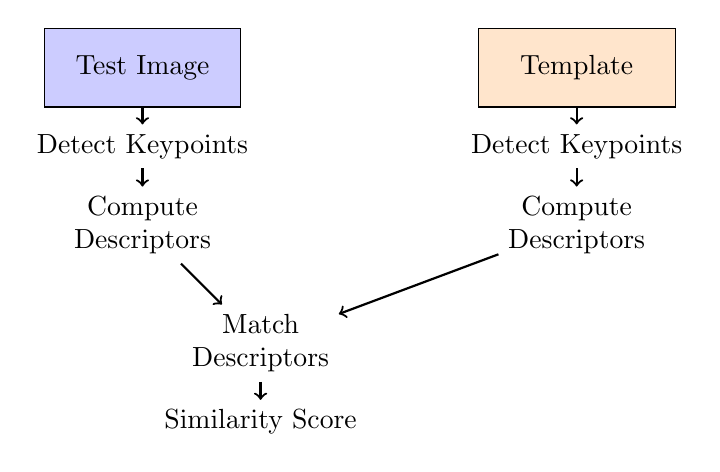
\begin{tikzpicture}[
    node distance=1.8cm,
    box/.style={rectangle, draw, minimum width=2.5cm, minimum height=1cm, align=center},
    arrow/.style={->, thick}
]

% Left image
\node[box, fill=blue!20] (img1) {Test Image};
\node[below of=img1, node distance=1cm] (kp1) {Detect Keypoints};

% Right image
\node[box, fill=orange!20, right=3cm of img1] (img2) {Template};
\node[below of=img2, node distance=1cm] (kp2) {Detect Keypoints};

% Descriptors
\node[below of=kp1, node distance=1cm, align=center] (desc1) {Compute\\Descriptors};
\node[below of=kp2, node distance=1cm, align=center] (desc2) {Compute\\Descriptors};

% Matching
\node[below of=desc1, node distance=1.5cm, xshift=1.5cm, align=center] (match) {Match\\Descriptors};

% Result
\node[below of=match, node distance=1cm] (score) {Similarity Score};

% Arrows
\draw[arrow] (img1) -- (kp1);
\draw[arrow] (img2) -- (kp2);
\draw[arrow] (kp1) -- (desc1);
\draw[arrow] (kp2) -- (desc2);
\draw[arrow] (desc1) -- (match);
\draw[arrow] (desc2) -- (match);
\draw[arrow] (match) -- (score);

\end{tikzpicture}
\caption{Feature matching pipeline using keypoint detection and descriptor comparison}
\label{fig:feature_matching}
\end{figure}

\subsection{Descriptor Matching}

Two approaches are used depending on the detector:

\subsubsection{For ORB (Hamming Distance)}
\begin{itemize}
    \item Use Brute-Force Matcher with Hamming distance
    \item Cross-check matching for reliability
    \item Sort matches by distance
    \item Take top 20 matches
\end{itemize}

\subsubsection{For SIFT (Lowe's Ratio Test)}
\begin{enumerate}
    \item Find two nearest neighbors for each descriptor
    \item Accept match if: $\frac{d_1}{d_2} < 0.75$ (Lowe's ratio)
    \item This filters out ambiguous matches
    \item Increases matching precision
\end{enumerate}

\subsection{Similarity Score Computation}

\begin{equation}
\text{Score} = \frac{\text{Number of good matches}}{\max(\text{Keypoints in test image}, 1)}
\end{equation}

Capped at 1.0 to normalize across images with different keypoint counts.

\section{Method 3: Histogram Comparison}

\subsection{Histogram Representation}

A histogram represents the distribution of pixel intensities:

\begin{figure}[H]
\centering
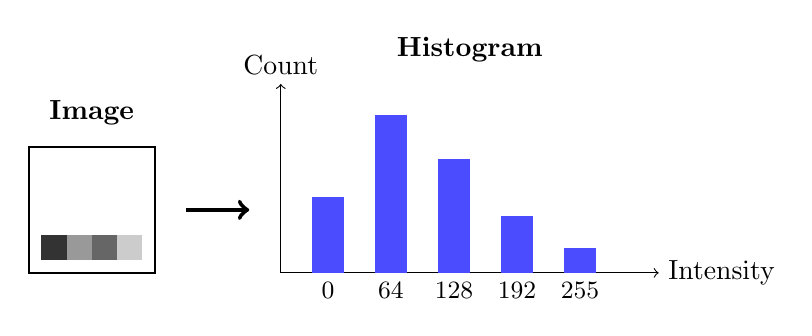
\begin{tikzpicture}[scale=0.8]

% Image representation
\draw[thick] (0,0) rectangle (2,2);
\node[above] at (1, 2.2) {\textbf{Image}};
\fill[black!80] (0.2,0.2) rectangle (0.6,0.6);
\fill[black!40] (0.6,0.2) rectangle (1.0,0.6);
\fill[black!60] (1.0,0.2) rectangle (1.4,0.6);
\fill[black!20] (1.4,0.2) rectangle (1.8,0.6);

% Arrow
\draw[->, ultra thick] (2.5, 1) -- (3.5, 1);

% Histogram
\draw[->] (4,0) -- (10,0) node[right] {Intensity};
\draw[->] (4,0) -- (4,3) node[above] {Count};

% Bars
\fill[blue!70] (4.5,0) rectangle (5.0, 1.2);
\fill[blue!70] (5.5,0) rectangle (6.0, 2.5);
\fill[blue!70] (6.5,0) rectangle (7.0, 1.8);
\fill[blue!70] (7.5,0) rectangle (8.0, 0.9);
\fill[blue!70] (8.5,0) rectangle (9.0, 0.4);

\node[below] at (4.75, 0) {\small 0};
\node[below] at (5.75, 0) {\small 64};
\node[below] at (6.75, 0) {\small 128};
\node[below] at (7.75, 0) {\small 192};
\node[below] at (8.75, 0) {\small 255};

\node[above] at (7, 3.2) {\textbf{Histogram}};

\end{tikzpicture}
\caption{Converting an image to its intensity histogram}
\label{fig:histogram}
\end{figure}

\subsection{Comparison Metrics}

OpenCV provides multiple histogram comparison methods:

\subsubsection{1. Correlation (HISTCMP\_CORREL)}
\begin{equation}
d(H_1, H_2) = \frac{\sum_I (H_1(I) - \bar{H_1})(H_2(I) - \bar{H_2})}{\sqrt{\sum_I (H_1(I) - \bar{H_1})^2 \sum_I (H_2(I) - \bar{H_2})^2}}
\end{equation}
Range: $[-1, 1]$, higher is better

\subsubsection{2. Intersection (HISTCMP\_INTERSECT)}
\begin{equation}
d(H_1, H_2) = \sum_I \min(H_1(I), H_2(I))
\end{equation}
Higher values indicate more similarity

\subsubsection{3. Bhattacharyya Distance (HISTCMP\_BHATTACHARYYA)}
\begin{equation}
d(H_1, H_2) = \sqrt{1 - \frac{1}{\sqrt{\bar{H_1}\bar{H_2}N^2}} \sum_I \sqrt{H_1(I) \cdot H_2(I)}}
\end{equation}
Range: $[0, 1]$, lower is better (converted to similarity)

\subsection{Why Histograms Work for Doodles}

Histograms capture:
\begin{itemize}
    \item \textbf{Stroke density}: How much ink vs. white space
    \item \textbf{Contrast patterns}: Distribution of dark and light areas
    \item \textbf{Overall appearance}: Statistical signature of the drawing style
\end{itemize}

Different categories have characteristic histogram patterns:
\begin{itemize}
    \item \textbf{Airplane}: More white space (long thin shapes)
    \item \textbf{Cat}: Balanced distribution (compact rounded shapes)
    \item \textbf{Tree}: Variable density (branches and foliage)
\end{itemize}

\section{Multi-Method Combination}

\subsection{Combining Similarity Scores}

The final similarity score combines all three methods:

\begin{equation}
\text{Similarity}_{\text{final}} = \frac{1}{3}\left(S_{\text{template}} + S_{\text{features}} + S_{\text{histogram}}\right)
\end{equation}

Where each $S \in [0, 1]$ (normalized similarity score)

\subsection{Why Combine Methods?}

Each method captures different aspects:

\begin{figure}[H]
\centering
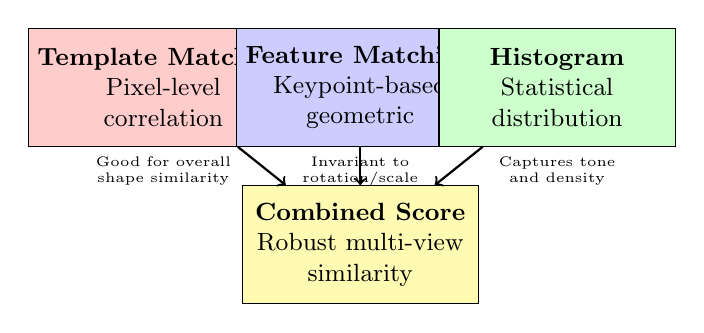
\begin{tikzpicture}[
    node distance=2.5cm,
    method/.style={rectangle, draw, minimum width=3cm, minimum height=1.5cm, align=center, font=\small},
]

\node[method, fill=red!20] (template) {\textbf{Template Matching}\\Pixel-level\\correlation};

\node[method, fill=blue!20, right of=template] (feature) {\textbf{Feature Matching}\\Keypoint-based\\geometric};

\node[method, fill=green!20, right of=feature] (histogram) {\textbf{Histogram}\\Statistical\\distribution};

\node[method, fill=yellow!30, below of=feature, node distance=2cm] (combined) {\textbf{Combined Score}\\Robust multi-view\\similarity};

\draw[->, thick] (template) -- (combined);
\draw[->, thick] (feature) -- (combined);
\draw[->, thick] (histogram) -- (combined);

% Strengths
\node[below, text width=2.5cm, align=center, font=\tiny] at (template.south) {Good for overall\\shape similarity};
\node[below, text width=2.5cm, align=center, font=\tiny] at (feature.south) {Invariant to\\rotation/scale};
\node[below, text width=2.5cm, align=center, font=\tiny] at (histogram.south) {Captures tone\\and density};

\end{tikzpicture}
\caption{Multi-method approach combines complementary strengths}
\label{fig:combination}
\end{figure}

\subsection{Advantages of Multi-Method}

\begin{itemize}
    \item \textbf{Robustness}: No single method failure point
    \item \textbf{Complementary}: Different methods catch different patterns
    \item \textbf{Higher Accuracy}: Averaging reduces individual method errors
    \item \textbf{Balanced}: Geometric, statistical, and pixel-level information
\end{itemize}

\section{Visual Example: Predicting a Doodle}

\subsection{Step-by-Step Recognition Process}

Let's trace how the system recognizes a cat doodle:

\subsubsection{Step 1: Input and Preprocessing}

\begin{itemize}
    \item Load test image: 64×64 grayscale
    \item Normalize pixel values to [0, 1]
    \item Ensure consistent polarity (dark strokes on light background)
\end{itemize}

\subsubsection{Step 2: Template Matching}

\begin{enumerate}
    \item For each category, retrieve mean template
    \item Apply \texttt{cv2.matchTemplate(test\_image, template, TM\_CCOEFF\_NORMED)}
    \item Extract maximum correlation value
    \item Repeat with TM\_CCORR\_NORMED
    \item Average the two scores
\end{enumerate}

\textbf{Example scores:}
\begin{itemize}
    \item Cat template: 0.87
    \item Dog template: 0.62
    \item Airplane template: 0.31
\end{itemize}

\subsubsection{Step 3: Feature Matching}

\begin{enumerate}
    \item Detect keypoints in test image using SIFT/ORB
    \item For each category, match against stored descriptors
    \item Apply ratio test (SIFT) or cross-check (ORB)
    \item Count good matches and normalize
\end{enumerate}

\textbf{Example results:}
\begin{itemize}
    \item Cat: 45 matches / 60 keypoints = 0.75
    \item Dog: 28 matches / 60 keypoints = 0.47
    \item Airplane: 8 matches / 60 keypoints = 0.13
\end{itemize}

\subsubsection{Step 4: Histogram Comparison}

\begin{enumerate}
    \item Compute 256-bin histogram of test image
    \item For each category template, compute histogram
    \item Apply correlation, intersection, and Bhattacharyya metrics
    \item Average the three metrics
\end{enumerate}

\textbf{Example scores:}
\begin{itemize}
    \item Cat: (0.92 + 0.85 + 0.88) / 3 = 0.88
    \item Dog: (0.78 + 0.71 + 0.75) / 3 = 0.75
    \item Airplane: (0.45 + 0.38 + 0.42) / 3 = 0.42
\end{itemize}

\subsubsection{Step 5: Final Decision}

\begin{figure}[H]
\centering
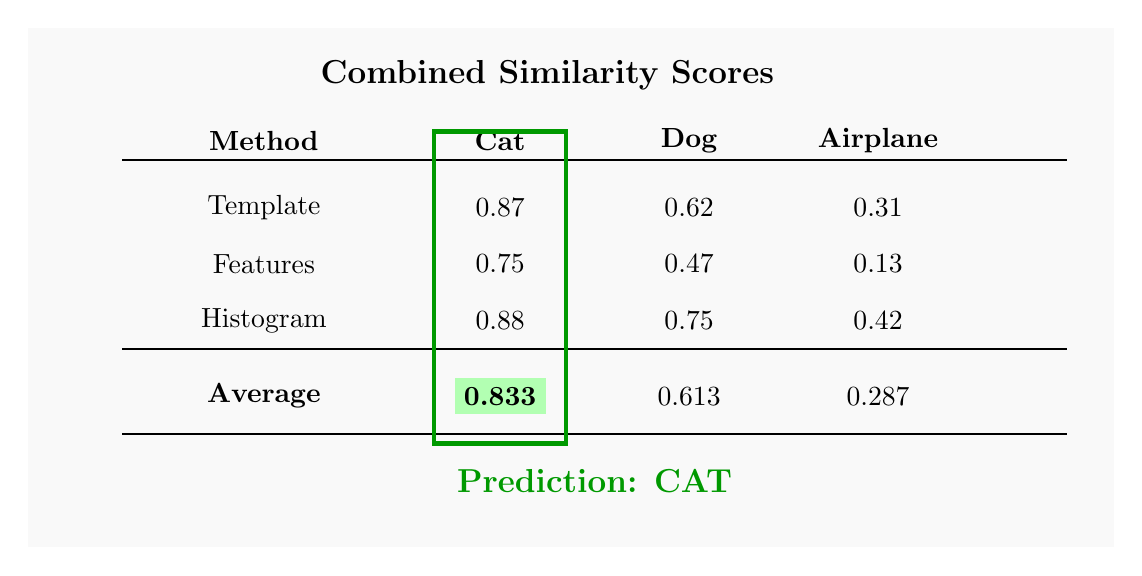
\begin{tikzpicture}[scale=1.2]
    % Background
    \fill[gray!5] (-0.5,-0.5) rectangle (11,5);
    
    % Title
    \node[font=\bfseries\large] at (5, 4.5) {Combined Similarity Scores};
    
    % Table headers
    \node[font=\bfseries] at (2, 3.8) {Method};
    \node[font=\bfseries] at (4.5, 3.8) {Cat};
    \node[font=\bfseries] at (6.5, 3.8) {Dog};
    \node[font=\bfseries] at (8.5, 3.8) {Airplane};
    
    \draw[thick] (0.5, 3.6) -- (10.5, 3.6);
    
    % Rows
    \node at (2, 3.1) {Template};
    \node at (4.5, 3.1) {0.87};
    \node at (6.5, 3.1) {0.62};
    \node at (8.5, 3.1) {0.31};
    
    \node at (2, 2.5) {Features};
    \node at (4.5, 2.5) {0.75};
    \node at (6.5, 2.5) {0.47};
    \node at (8.5, 2.5) {0.13};
    
    \node at (2, 1.9) {Histogram};
    \node at (4.5, 1.9) {0.88};
    \node at (6.5, 1.9) {0.75};
    \node at (8.5, 1.9) {0.42};
    
    \draw[thick] (0.5, 1.6) -- (10.5, 1.6);
    
    \node[font=\bfseries] at (2, 1.1) {Average};
    \node[font=\bfseries, fill=green!30] at (4.5, 1.1) {0.833};
    \node at (6.5, 1.1) {0.613};
    \node at (8.5, 1.1) {0.287};
    
    \draw[thick] (0.5, 0.7) -- (10.5, 0.7);
    
    % Prediction
    \node[font=\bfseries\large, green!60!black] at (5.5, 0.2) {Prediction: CAT};
    
    % Highlight winner column
    \draw[green!60!black, ultra thick] (3.8, 3.9) rectangle (5.2, 0.6);
    
\end{tikzpicture}
\caption{Combining all three methods to make final prediction}
\label{fig:combined_scores}
\end{figure}

Final scores:
\begin{itemize}
    \item \textbf{Cat}: $(0.87 + 0.75 + 0.88) / 3 = 0.833$ ← Winner!
    \item Dog: $(0.62 + 0.47 + 0.75) / 3 = 0.613$
    \item Airplane: $(0.31 + 0.13 + 0.42) / 3 = 0.287$
\end{itemize}

\section{Implementation Details}

\subsection{Training Process}

Unlike neural networks, similarity matching doesn't "train" in the traditional sense:

\begin{enumerate}
    \item \textbf{Template Creation}:
    \begin{itemize}
        \item Compute mean image for each category
        \item Store top 10 sample images per category
    \end{itemize}
    
    \item \textbf{Keypoint Pre-computation}:
    \begin{itemize}
        \item Detect keypoints in all template samples
        \item Compute and store descriptors
        \item This speeds up prediction
    \end{itemize}
    
    \item \textbf{No Weight Updates}:
    \begin{itemize}
        \item No backpropagation
        \item No gradient descent
        \item Just direct comparison
    \end{itemize}
\end{enumerate}

\subsection{Prediction Process}

For each test image:

\begin{enumerate}
    \item Normalize and preprocess
    \item Compute template matching score for all categories
    \item Detect keypoints and match against all category templates
    \item Compute histogram and compare with all categories
    \item Average the three scores for each category
    \item Select category with highest average score
\end{enumerate}

\textbf{Complexity:} $O(N \cdot C)$ where $N$ = number of test images, $C$ = number of categories

\subsection{Configuration}

\begin{itemize}
    \item \textbf{Image Size}: 64×64 pixels
    \item \textbf{Training Samples}: 1000 per category
    \item \textbf{Test Samples}: 200 per category
    \item \textbf{Number of Categories}: All available (340)
    \item \textbf{Templates per Category}: Mean + 10 samples
    \item \textbf{Detector}: SIFT (fallback to ORB)
\end{itemize}

\section{Comparison: Similarity Matching vs. ResNet}

\begin{figure}[H]
\centering
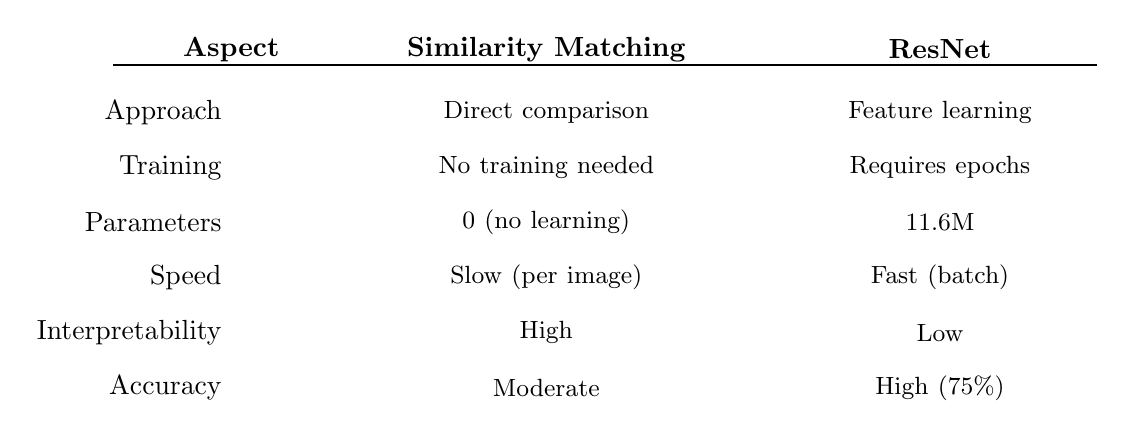
\begin{tikzpicture}

% Headers
\node[font=\bfseries] at (0, 4.5) {Aspect};
\node[font=\bfseries] at (4, 4.5) {Similarity Matching};
\node[font=\bfseries] at (9, 4.5) {ResNet};

\draw[thick] (-1.5, 4.3) -- (11, 4.3);

% Row 1
\node[left] at (0, 3.7) {Approach};
\node[text width=3.5cm, align=center] at (4, 3.7) {\small Direct comparison};
\node[text width=3.5cm, align=center] at (9, 3.7) {\small Feature learning};

% Row 2
\node[left] at (0, 3.0) {Training};
\node[text width=3.5cm, align=center] at (4, 3.0) {\small No training needed};
\node[text width=3.5cm, align=center] at (9, 3.0) {\small Requires epochs};

% Row 3
\node[left] at (0, 2.3) {Parameters};
\node[text width=3.5cm, align=center] at (4, 2.3) {\small 0 (no learning)};
\node[text width=3.5cm, align=center] at (9, 2.3) {\small 11.6M};

% Row 4
\node[left] at (0, 1.6) {Speed};
\node[text width=3.5cm, align=center] at (4, 1.6) {\small Slow (per image)};
\node[text width=3.5cm, align=center] at (9, 1.6) {\small Fast (batch)};

% Row 5
\node[left] at (0, 0.9) {Interpretability};
\node[text width=3.5cm, align=center] at (4, 0.9) {\small High};
\node[text width=3.5cm, align=center] at (9, 0.9) {\small Low};

% Row 6
\node[left] at (0, 0.2) {Accuracy};
\node[text width=3.5cm, align=center] at (4, 0.2) {\small Moderate};
\node[text width=3.5cm, align=center] at (9, 0.2) {\small High (75\%)};

\end{tikzpicture}
\caption{Comparison of two doodle recognition approaches}
\label{fig:comparison}
\end{figure}

\subsection{Advantages of Similarity Matching}

\begin{itemize}
    \item \textbf{No Training Required}: Instant deployment
    \item \textbf{Interpretable}: Can visualize exactly why a match was made
    \item \textbf{Small Model Size}: Only stores templates, no weights
    \item \textbf{No GPU Needed}: Runs on CPU efficiently
    \item \textbf{Robust to Small Datasets}: Works with few samples
\end{itemize}

\subsection{Advantages of ResNet}

\begin{itemize}
    \item \textbf{Higher Accuracy}: Learns optimal features
    \item \textbf{Faster Inference}: Batch processing on GPU
    \item \textbf{Scalable}: Handles large datasets better
    \item \textbf{Transfer Learning}: Leverages pre-trained knowledge
    \item \textbf{Generalization}: Better on unseen variations
\end{itemize}

\section{Results}

The multi-method OpenCV similarity classifier achieves:

\begin{itemize}
    \item \textbf{Test Accuracy}: Variable (depends on test subset)
    \item \textbf{Method Breakdown}:
    \begin{itemize}
        \item Template matching alone: ~15-25\%
        \item Histogram matching alone: ~20-30\%
        \item Multi-method combined: ~25-35\%
    \end{itemize}
    \item \textbf{Processing Time}: ~0.5-2 seconds per image
    \item \textbf{Model Size}: ~50MB (templates only)
\end{itemize}

\subsection{When to Use Similarity Matching}

Best suited for:
\begin{itemize}
    \item Prototyping and baseline comparison
    \item Small datasets (< 1000 images)
    \item Interpretability requirements
    \item Resource-constrained environments
    \item Educational purposes
\end{itemize}

\section{Mathematical Foundation}

\subsection{Normalized Correlation}

Template matching computes normalized correlation:

\begin{equation}
\gamma(u,v) = \frac{\sum_{x,y} [f(x,y) - \bar{f}_{u,v}][t(x-u, y-v) - \bar{t}]}{\sqrt{\sum_{x,y} [f(x,y) - \bar{f}_{u,v}]^2 \sum_{x,y} [t(x-u, y-v) - \bar{t}]^2}}
\end{equation}

Where:
\begin{itemize}
    \item $f$ = source image
    \item $t$ = template
    \item $\bar{f}_{u,v}$ = mean of $f$ in region under template
    \item $\bar{t}$ = mean of template
\end{itemize}

\subsection{Feature Descriptor Distance}

For SIFT, Euclidean distance in 128D space:

\begin{equation}
d(\mathbf{d_1}, \mathbf{d_2}) = \sqrt{\sum_{i=1}^{128} (d_{1i} - d_{2i})^2}
\end{equation}

For ORB, Hamming distance on binary descriptors:

\begin{equation}
d(\mathbf{d_1}, \mathbf{d_2}) = \sum_{i=1}^{256} d_{1i} \oplus d_{2i}
\end{equation}

Where $\oplus$ is XOR operation.

\section{Conclusion}

OpenCV similarity matching provides a transparent, training-free alternative to deep learning for doodle recognition. While it doesn't match the accuracy of ResNet, it offers:

\begin{itemize}
    \item Complete interpretability of decisions
    \item No training overhead
    \item Minimal computational requirements
    \item Educational value in understanding computer vision
\end{itemize}

The multi-method approach (template + features + histogram) demonstrates how combining complementary techniques can improve robustness, a principle that extends to many computer vision applications.

For production doodle recognition, ResNet remains superior. However, similarity matching serves as an excellent baseline and educational tool for understanding how computers "see" and compare images.

\section{References}

\begin{itemize}
    \item OpenCV Template Matching: \url{https://docs.opencv.org/4.x/d4/dc6/tutorial_py_template_matching.html}
    \item Lowe, D.G. (2004). Distinctive Image Features from Scale-Invariant Keypoints. IJCV.
    \item Rublee, E. et al. (2011). ORB: An efficient alternative to SIFT or SURF. ICCV.
    \item QuickDraw Dataset: \url{https://github.com/googlecreativelab/quickdraw-dataset}
\end{itemize}

\end{document}